\documentclass[12pt,a4paper]{article}
\usepackage{times}
\usepackage[utf8]{inputenc}
\usepackage[lmargin=2.5cm, rmargin=2.5cm, tmargin = 2.5cm, bmargin = 2.5cm]{geometry}
\usepackage[czech]{babel}
\usepackage{graphicx}
\usepackage{setspace}
\usepackage{amsmath}
\usepackage[hidelinks]{hyperref}
\usepackage{siunitx}
\usepackage{mhchem}
\usepackage{multirow}
\usepackage{pdflscape}
\usepackage{changepage}
\usepackage{float}
\usepackage{xurl}
\newcommand{\citovano}{[cit. 2022-04-25] }

\sisetup{
	round-mode = places,
	round-precision = 6,
	round-pad = false,
	output-decimal-marker={,}
}
\newcommand{\e}{$e^-$}
%from https://tex.stackexchange.com/questions/48152/signature-date-line-with-fixed-width
\usepackage{xparse}
\makeatletter
\newcommand*\signaturelinewidth{5cm}
\newcommand*\signaturelineheight{.4pt}
\newcommand*\signaturedashleaderatom{\kern .1pt.\kern .1pt}
\newcommand*\signaturelineraise{.4ex}
\newcommand*\signaturelabelindent{.5cm}
\newcommand*\signaturetextindent{}
\NewDocumentCommand\signatureline{
	O{\signaturelinewidth}      % line width
	O{\signaturelabelindent}    % label margin
	O{%                           text indentation
		\ifx\@empty\signaturetextindent
		.5\dimexpr #2\relax
		\else
		\signaturetextindent
		\fi
	}
	m                           % label
	O{\signaturelineheight}     % line height
	O{\signaturelineraise}      % line raise
	D||{}                       % text
}{%
	\parbox[t]{#1}{%
		\leftskip #3%
		\mbox{\strut #7}%
		\vskip -#6%
		\hrule height #5%
		\vskip #6%
		\scriptsize
		\leftskip #2%
		\rightskip #2%
		\strut #4%
	}%
}
\NewDocumentCommand\signaturedash{
	O{\signaturelinewidth}      % line width
	O{\signaturelabelindent}    % label margin
	O{%                           text indentation
		\ifx\@empty\signaturetextindent
		.5\dimexpr #2\relax
		\else
		\signaturetextindent
		\fi
	}
	m                           % label
	O{\signaturedashleaderatom} % leader atom
	O{\signaturelineraise}      % line raise
	D||{}                       % text
}{%
	\parbox[t]{#1}{%
		\leftskip #3%
		\mbox{\strut #7}%
		\vskip -#6%
		\leftskip 0pt%
		\hrule height 0pt%
		\leavevmode\cleaders\hbox{#5}\hfill\kern 0pt%
		\hrule height 0pt%
		\vskip #6%
		\scriptsize
		\leftskip #2%
		\rightskip #2%
		\strut #4%
	}%
}

\begin{document}
\begin{spacing}{1.5}
\begin{titlepage}
	\begin{center}
		\large
		\textbf{Střední průmyslová škola a Vyšší odborná škola Brno, Sokolská,
			příspěvková organizace}\\
		\vspace*{4.5cm}
		\Huge
		ROČNÍKOVÁ PRÁCE\\
		z Fyziky\\
		\vspace*{4.5cm}
		\LARGE
		\textbf{Kalibrace HPGe detektoru}
		\vspace{1.5cm}
		
		\vfill
		\vspace{0.8cm}
		\large
		\begin{tabular}{p{0.2\textwidth} p{0.8\textwidth}}
			Studijní obor:& Technické lyceum 78 – 42 - M/01\\
			Třída:& L3A\\
			Školní rok:& 2021/2022\\
			Jméno:& \textbf{David}\\
			Příjmení:& \textbf{Škrob}\\
		\end{tabular}
	\end{center}
\end{titlepage}
\pagestyle{empty}
\vspace*{\fill}\hspace*{-20pt}
\textbf{Prohlašuji, že jsem tuto práci vypracoval samostatně a použil jsem literárních
	pramenů a~informací, které cituji a uvádím v seznamu použité literatury a zdrojů
	informací.}\\ 
\vspace{.2cm}\\%tohle jsem zmenil
\makeatother
	V Brně dne :
	\signaturedash[3cm]{}\hspace*{7cm}
	\signaturedash[3cm]{David Škrob}
\newpage
\tableofcontents
\newpage
\pagestyle{plain}
\setcounter{page}{3}
% Jen Aby to bylo fancy
%pod záštitou
%
\includegraphics[width=0.1\textwidth]{vut.jpg}
\addcontentsline{toc}{section}{Zadání}
\section*{Zadání}
Popište jak funguje polovodičová detekce gama záření. Pomocí sady kalibračních zářičů stanovte účinnost detekce gama záření HPGe (High Purity Germanium) detektorem pro vybranou měřící pozici. Pomocí statistických metod a teoretických znalostí určete, s čím ztráty souvisí. % Změřené a vypočtené efektivity proložte vhodnou funkcí. Pomocí statistických metod nalezněte nejvhodnější stupeň fitu vybranou funkcí.
\newpage
\addcontentsline{toc}{section}{Úvod}
\section*{Úvod}%TODO napsat celej uvod znova{res. ta prvni odrazka je asi jednia dobra...}
Gama záření je vysokoenergetické elektromagnetické záření, které vzniká v jádru atomu při radioaktivních přeměnách. Rozdíl mezi zářením gama a zářením rentgenovým je v původu záření. Rentgenové záření vzniká v atomovém obalu, a má většinou nižší energii (\SI{1}{\kilo\electronvolt} až\SI{6000}{\kilo\electronvolt} v extrémnínch připadech až \SI{6000}{\kilo\electronvolt}). Gama záření pochází z atomvého jádra, má vyšší energie (\SI{100}{\kilo\electronvolt}, ale někdy i tak málo jako \SI{0.007}{\kilo\electronvolt}).\\%gama - thorium 229m, rtg - muonovy atom
%jak se meri
%pridat proc se to co delam normalne dela
Gama záření můžeme měřit buď pouze bez rozlišení, například Geigerův–Müllerův počítačem, nebo můžeme měřit energii dopadajících fotonů, třeba pomocí scintilačních detektorů, nebo detektorů polovodičových, jako je HPGe.\\
Tato ročníková práce se bude zabývat vlivem ztráty signálu gama záření v závislosti na vzdálenosti. Bude se též zabývat rozlišovací schopností detektoru při různých energiích fotonu. Snaha této práce je najít takové funkce, aby bylo možné tyto vlivy odfiltrovat při měření neznámého vzorku.\\
%Vezmu kalibrační vzorek, dám jej na detektor, počkám, dokud v peaku nebude 10~000 záznamů. Poté kalibrační vzorek schovám zpět do trezoru. Následně budu analyzoval daná data a z nich jsem vytvořil příslušné grafy.\\
%spektroskopie
%\footnote{https://www.ortec-online.com/-/media/ametekortec/technical\%20papers/homeland\%20security\%20applications\%20and\%20chemical\%20weapons\%20assay\%20pins/whyhighpuritygermaniumhpgeradiationdetectiontechnologysuperiorotherdetectortechnologiesisotopeidentification.pdf?la=en}
\newpage
\section{Detekce ionizujícího záření}
Hlavním důvodem, proč se používají HPGe detektory: 
Jsou lépe schopné určit, o jakou energii se jedná, čehož můžeme využít při rozlišování jednotlivých radioaktivních izotopů. Tak můžeme zjistit, zda se v přepravě radioaktivních materiálů nesnaží někdo přepravit speciální jaderný materiál, který by mohl být použit na výrobu jaderných zbraní \cite{isotopeIdent}.\\ 
%to je nejak navic
%Byli použity referenční zdroje gama záření, u kterého jsou známy jeho energie, abychom mohli detektor zkalibrovat \cite{jirka_burian_bakalarka}.
%\footnote{https://www.vut.cz/www\_base/zav\_prace\_soubor\_verejne.php?file\_id=195526}%rozbyte
HPGe detektory mají vyšší tepelný šum, který by při pokojové teplotě přehlušil měřený signál. Potřebují taky napétí v řádu \SI{}{\kilo\volt}, které by jsme při pokojové teplotě nemohly použít. Proto jej chladíme kapalným dusíkem na teplotu \SI{-196}{\degreeCelsius} \cite{comprarsion,zlin2010}.\\ %\footnote{Zlín 2011 SENZORY.} 
 %\footnote{https://www.radiation-dosimetry.org/what-is-advantage-and-disadvantage-of-germanium-detectors-definition/}
Energii z dopadajících fotonů můžeme detekovat nejen pomocí fotoelektrického jevu, ale taky pomocí 2 dalších jevů. Tyto jevy jsou ovšem spíše jako parazitní, protože často se nepohltí celá energie fotonu.\\
\subsection{Detekce fotoelektrického jevu}
Když se do citlivé vrstvy detektoru (u germania díky speciální technice výroby velmi čistého germania v řádu \SI{}{\centi\meter}, u křemíku v řádu \SI{}{\milli\meter})  \cite{Knoll2010} %\footnote{G.F: Knoll str 415}
dostane $\gamma$ foton, tak díky fotoelektrickému jevu gama foton uvolní \e z elektronového obalu. Asi \SI{3}{\electronvolt} jsou potřeba na uvolnění \e z valenční vrstvy. (V případě Germania asi \SI{3,6}{\electronvolt}, v případě křemíku asi \SI{2,9}{\electronvolt}) \cite{astrnukleofyzika, nuclear_power-hpge}.\\ %\footnote{https://astronuklfyzika.cz/DetekceSpektrometrie.htm}
%\footnote{https://www.nuclear-power.com/nuclear-engineering/radiation-detection/semiconductor-detectors/high-purity-germanium-detectors-hpge/principle-of-operation-of-hpge-detectors}
Tato energie je nutná na odtržení \e od atomu. Zbylá energie gama fotonu se stane kinetickou energií \e. \uv{V polovodiči fotoelektron ztratí svou kinetickou energii při interakci elektromagnetickými silami s elektrony v polovodičové mřížce, čímž vzniká mnoho párů elektron-díra. Počet vytvořených párů elektron-děr je přímo úměrný energii dopadajícího fotonu.} \cite{semiconductors} %\footnote{Semiconductors for Room Temperature Nuclear Detector Applications, str. 23}%Albert Beer, Robert Willardson, Eicke Weber
Na diodu detektoru přivedeme v závěrném směru napětí, řadově tisíce~\SI{}{\volt} \cite{hpge-detector_fabrication}. %\footnote{https://sci-hub.se/10.1109/TNS.1972.4326520}
Jakmile se vytvoří pár \e~díra, tak se \e  přesouvá ke kladně nabité elektrodě, díra k záporně nabité, vzniká proud, a ten potom zaznamenáváme \cite{VUT,Knoll2010}. 
\subsection{Detekce Comptnova jevu}
Prvním z nich je Comptonův jev, kde gama foton část své energie předá \e , který je vychýlen ze své původní dráhy. Foton změní směr pohybu a zvýší se jeho vlnová délka. \cite{robert_macku}
Tento foton může dále reagovat v detektoru, až dokud se nedostane mimo citlivou vrstvu detektoru, \break nebo dokud není zcela pohlcen.\\
\subsection{Detekce páru pozitron-elektron}
Druhým z nich je tvorba páru elektron-pozitron, kdy pokud se $\gamma$ foton přiblíží k jádru atomu, tak se z jeho energie vytvoří pár \e, $e^+$. Musí se vytvořit oba, aby platil zákon zachování náboje. Jejich vytvoření neporušuje zákon zachování hmoty, protože platí teorie relativity, \break ze které vyplývá:  
\begin{equation}
	%https://opentextbc.ca/universityphysicsv3openstax/chapter/relativistic-energy/
	E^2 = (mc^2)^2 + (pc)^2
\end{equation}
Kde $E$ je energie fotonu, $m$ je hmotnost \e a $e^+$, kteří se vytvoří a $p$ je hybnost, která je rozdělena mezi ně a jádro atomu, u kterého se tato přeměna stane. 
Pokud měl foton větší energii než \SI{1022}{\kilo\electronvolt} ($m_{e} = \SI{9.1093837e-31}{\kilogram}$, $E=mc^2 \implies E = \SI{9.1093837e-31}{\kilogram} \cdot [\SI{299792458}{\meter\per\second}]^2 = \SI{8.1871058e-14}{\joule} =~\SI{510.999}{\kilo\electronvolt}$\footnote{\SI{}{\electronvolt} je jednotka energie, je definována jako kinetická energie, kterou ve vakuu \e dostane  při urychlení napětím \SI{1}{\volt}. Energie komára je \SI{1e12}{\electronvolt}, jednotka je proto využívána v místech, kde jsou energie velmi malé, jako například v částicové fyzice.}, je energie \e a protože vytváříme pár \e a $e^+$, potřebujeme 2 násobnou energii tj.~$\SI{1021.998}{\kilo\electronvolt}$).\enlargethispage{\baselineskip} Pokud má $\gamma$ záření větší energii, tak tato energie je převedena na hybnost \e a $e^+$ \cite{semiconductors,libretext_pair}. %\footnote{ https://phys.libretexts.org/@go/page/10492} 
%\footnote{Semiconductors for Room Temperature, str. 23} 
\section{Měření účinnosti}%dost souvisi z kalibraci
Tato kapitola se bude zabývat, jaké vlivy má energie dopadajícího $\gamma$ fotonu. Jak působí energie na rozlišovací schopnost detektoru a jakým způsobem energeticky kalibrujeme detektor. 
\subsection{Vliv energie}
U vlivu energie řešíme, jaké rozlišení má detektor při dané energii. Používáme při tom FWHM, kde můžeme snadno určit, jak je peak široký, a kdy by nám již 2 peaky splynuly v jeden \cite{stellarnet-fwhm, VUT}.\\ %\footnote{https://www.stellarnet.us/what-is-full-width-at-half-maximum-fwhm/} 
\uv{Systémy s malým germaniovým detektorem mají FWHM přibližně 150-250 eV při 5,9 keV, kdy se FWHM zvyšuje na 400-600 eV při 122 keV. Větší koaxiální detektory mají hodnoty FWHM mezi \SI{0.8}{\kilo\electronvolt} až \SI{1.2}{\kilo\electronvolt} při \SI{122}{\kilo\electronvolt}, kdy se zvýší na \SI{1.7}{\kilo\electronvolt} až \SI{2.3}{\kilo\electronvolt} při \SI{1333}{\kilo\electronvolt}.} \cite{Knoll2010} %\footnote{str. 428}
%https://www.nuclear-power.com/nuclear-power/reactor-physics/interaction-radiation-matter/interaction-gamma-radiation-matter/ ??

%dodat ze par positron neutron muze delat blbosti
\subsection{Energetická kalibrace detektoru}
Při kalibraci jsem použil software GAMWIN, který je určený na~ovládání a~kalibraci gama detektorů. K změřeným kalibračním vzorkům (\ce{^{241}Am}, \ce{^{57}Co}, \ce{^{60}Co}, \ce{^{137}Cs}, \ce{^{88}Y}, \ce{^{65}Zn}) jsem našel na \textit{Database WWW Table of Radioactive Isotopes}\footnote{\url{http://nucleardata.nuclear.lu.se/toi/nucSearch.asp}}
jejich energie gama rozpadu. Tyto energie jsem přiřadil k datům, která jsem naměřil, a~program GAMWIN tyto data proložil vhodnou funkcí. \cite{VUT,gamwin} 
%\footnote{https://www.nuviatech-instruments.com/cz/Produkt/nusoft-gamwin/}
\subsection{Výpočet efektivity detektoru}
\begin{figure}[h!]
	\renewcommand\figurename{Graf}
	\centering
	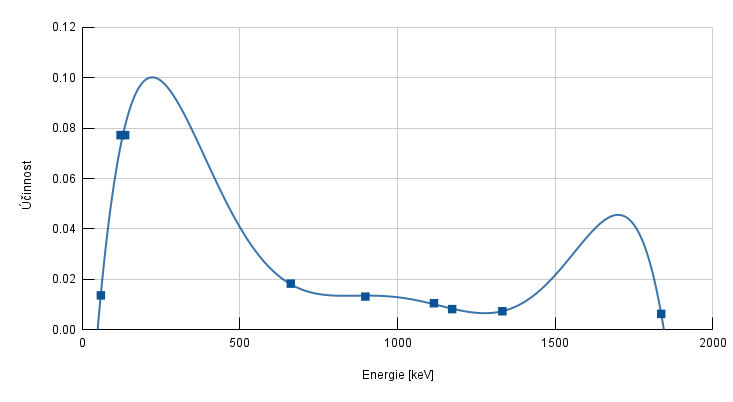
\includegraphics[width=0.7\linewidth]{google1.png}%mel by byt popis toho grafu "2x"
	\caption{Závislost účinnosti na energii, pro pozici \SI{5}{\milli\metre} nad detektorem.}
	\label{fig:EFFvsENG5mm}
\end{figure}
Na výpočet efektivity detektoru, jsem použil rovnici  (\ref{eqn:effectivity}), která určí pro danou energii peakovou účinnost.
 %První člen je zde pro počítaní efektivity.
 Druhý člen je na kompenzaci pro přeměnu mezi referenčním datem a datem měření. Třetí člen je zde pro kompenzaci přeměny během měření. %korekci/kompenzaci
\begin{equation}
	\label{eqn:effectivity}
	\varepsilon = \frac{S_{peaku}\lambda\frac{t_{real}}{t_{live}}}{A_0 I_\gamma}\cdot\frac{1}{e^{-\lambda t_0}}\cdot\frac{1}{1-e^{-\lambda t_{real}}}
\end{equation}
Kde $\varepsilon$ je peaková účinnost, $S_{peaku}$ je plocha peaku, bez plochy radiačního pozadí, $\lambda$ poločas přeměny  $t_{real}$ je doba, jak dlouho probíhalo celé měření, $t_{live}$ doba, jak dlouho detektor měřil (doba měření bez mrtvé doby detektoru), $A_0$ referenční aktivita kalibračního zdroje,  $I_\gamma$ je tabulková intenzita kalibračního zdroje a $t_0$ je doba mezi měřením a měřením referenční aktivity.
\section{Rozdíly při měření v různých vzdálenostech}
Měříme v různých vzdálenostech protože v nízké geometrii může intenzivní vzorek zahltit detektor, a v vysoké geometrii může málo intenzivní vzorek být téměř nepatrný. 
\subsection{Teoretický pokles intenzity}
Jak dobře známe, tak platí zákon převrácených čtverců, který nám říká, že intenzita klesá se čtvercem vzdálenosti.
\begin{equation}
	\frac{I_1}{I_2} = \frac{h_1^2}{h_2^2} \implies I_1 = I_2 \cdot \frac{h_1^2}{h_2^2}
\end{equation}
Kde $I_1$ je intenzita v bodě 1, $I_2$ je intenzita v bodě 2, $h_1^2$ vzdálenost bodu 1 od zdroje a $h_2^2$ vzdálenost bodu 2 od zdroje.\\
I přes to, že neměříme ve vakuu a vzorek pokládáme na plastovou destičku, tak tyto ztráty zanedbáme, protože budou mnohonásobně menší než ztráty způsobené zákonem převrácených čtverců. Například abychom ztratili polovinu fotonů o energii \SI{100}{\kilo\electronvolt}, tak bychom potřebovali \SI{35}{\meter} vysoký sloup vzduchu \cite{nuclear_power-gama_radiation}. %\footnote{https://www.nuclear-power.com/nuclear-power/reactor-physics/interaction-radiation-matter/interaction-gamma-radiation-matter/}
\subsection{Skutečná ztráta intenzity}
\begin{figure}[h]
	\renewcommand\figurename{Graf}
	\centering
	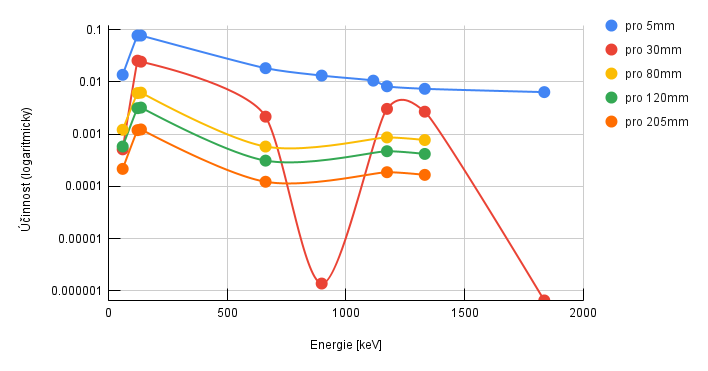
\includegraphics[width=\linewidth]{google2.png}
	\caption{Porovnání závislosti účinnosti na energii při různých vzdálenostech, kde osa y je logaritmická.}
	\label{fig:EFFvsENGvsDIS}
\end{figure} 
Na grafu \ref{fig:EFFvsENGvsDIS} vidíme, že účinnost se vzdáleností rychle klesá. Dále si můžeme povšimnout, \break že citlivost na energii zůstává stejná, takže pokles účinnosti je zde závislý na vzdálenosti.%mozna graf kde fitnu to jak ta ucinosionizující zářenít pada se vzdáleností
\section{Jiné vlivy na měření ionizujícího záření}
Při měření na HPGe detektoru si musíme dát pozor i na jiné vlivy, jako je například koincidenční detekce fotonů a přirozené radiační pozadí. Také měření ovlivní konstrukce detektoru a s tím související jeho mrtvá doba
\subsection{Mrtvá doba detektoru}
%detektor meri live time, a all time, z cehos dopocitame mrtvou dobu
Mrtvá doba detektoru, je doba, kdy detektor není citlivý na detekci dalšího fotonu. Při měření ji vyjadřujeme jako procentní podíl z celkového času měření.\\
Dělíme ji na nekumulativní a kumulativní. \\
Nekumulativní - foton, který není registrován, nemá vliv na samotný detektor. Většinou je způsobena tím, že detekční člen dokáže registrovat fotony rychleji než elektronika stíhá zpracovávat signál \cite{VUT}. %stíha ? je to dobry slovo
\begin{equation}
	n = \frac{N}{1+N*\tau}
\end{equation}
Kde $n$ je počet registrovaných fotonů, $N$ je počet fotonů, které zasáhly detektor a  $\tau$ je mrtvá doba detektoru, definovaná jako doba, po kterou detektor není schopen zaznamenat další foton.\\
Kumulativní - foton, který není registrován, prodlouží mrtvou dobu detektoru. Je způsobena tím, že je přehlcen detekční člen. Při zvyšování četnosti je zpočátku odezva téměř lineární, \break při dalším navýšení četnosti počet registrovaných impulzů začne klesat \cite{VUT}. 
\begin{equation}
	n = N \cdot e^{-N*\tau}
\end{equation}
\begin{figure}[H]
	\centering
	\setcounter{figure}{0}
	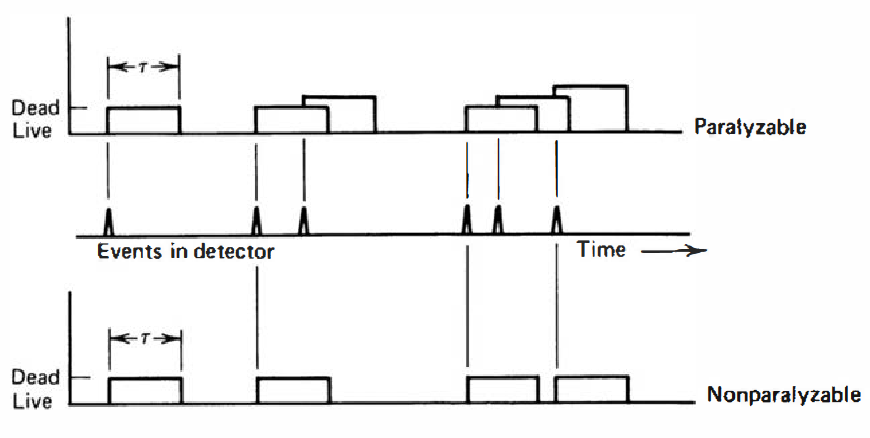
\includegraphics[width=0.8\textwidth]{fig1.png}
	%vzal jsem to z Glenn F. Knoll str 122
	%vut - str 21
	\caption{ Kumulativní (nahoře) a nekumulativní (dole) mrtva doba. Zdroj: \cite{Knoll2010}}
\end{figure}
Mrtvou dobu můžeme měřit několika způsoby, mezi nejrozšířenější patří \uv{metoda postupného oddalování (nebo přibližování) zdroje, až dokud není dosažena maximální četnost, kterou je detektor schopen měřit. Další zvyšovaní četnosti již nevede k zvyšování počtu zaznamenaných impulzů.}  \cite{VUT} %\footnote{Jaderně energetická zařízení -Laboratorní cvičení str.22}
%\subsection{Koincidenční detekce fotonů}
%V případě, že při měření vidíme, že se nám tvoří peak, v místě, které je dvojnásobkem 
%Glenn F. Knoll 440
\subsection{Radiační pozadí}
V Zemské kůře jsou radioaktivní prvky, které vyzařují gama záření. Z vesmíru se při různých dějích vytváří $\gamma$ záření. Tato záření jsou sice málo intenzivní, přesto vytváří šum na detektoru. \\
\begin{figure}[h!]
	\centering
	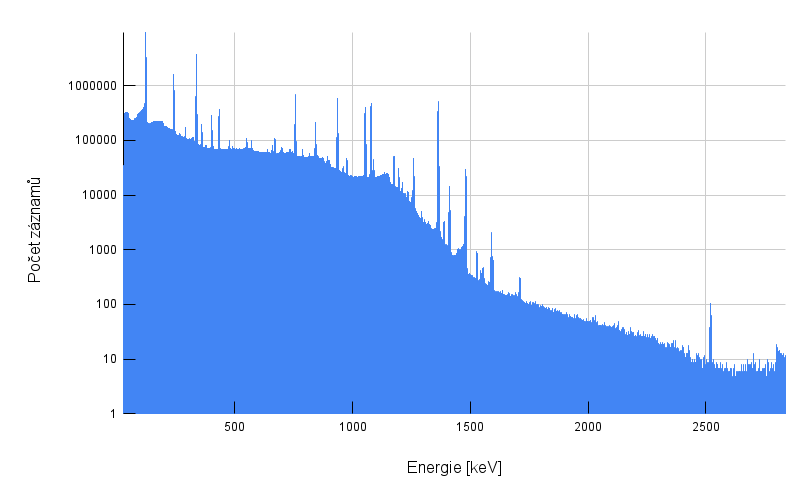
\includegraphics[width=0.75\textwidth]{pozadi_google.png}
	%z vlastniho merení
	\label{fig:pozadi}
	\caption{Spektrum měření přirozeného pozadí. Zdroj dat: Dušan Král}% 
\end{figure}\\
%\ref{fig:pozadi} 
%Na obrázku 2 vidíme, že nejvyšší naměřená hodnota je zhruba 540 záznamů. Toto pozadí jsem měřil 2 dny, takže to znamená, že detektor je dobře odstíněný.
%\section*{Poznámky a odkazy}
\addcontentsline{toc}{section}{Závěr}
\section*{Závěr}%prvni veta ? spis mozna uplne prepsat

Díky mé ročníkové práci jsem si mohl prohlédnout na Fakultu elektrotechniky a komunikačních technologií VUT. Povedlo se mi detektor nakalibrovat v programu \mbox{GAMWIN} a spočítat jeho efektivitu. Ale pro přesnějši kalibraci, bych potřeboval naměřit vzorek s zářením o energii asi \SI{500}{\kilo\electronvolt}. Kalibraci HPGe detektoru jsem dělal, abych mohl při navazující maturitní práci využit energetickou kalibraci pro určování energii k odpovídajícím peakům. A abych byl schopen určit, jakou má vzorek intenzitu, díky peakové účinnosti. Se stářím detektoru a měnícím se podmínkám v laboratoři je potřeba dělat tuto kalibraci a určování peakové účinnosti.


% to je popis prace, ne zaver ??asi??
%Vždy jsem počkal, dokud jsem neměl v nejvyšším bodě alespoň \num{10000} záznamů. Následně jsem data z těchto měření energeticky analyzoval, abych byl schopný určit, jaká energie přísluší kterému kanálu. %chanel
%Poté jsem analyzoval účinnost detektoru, pro 5 různých pozic, a tyto účinnosti jsem následně vynesl do grafu. 

\newpage
\addcontentsline{toc}{section}{Seznam použitých značek a symbolů}
\section*{Seznam použitých značek, symbolů a zkratek}
\begin{spacing}{1.2}
	\begin{list}{}{}
		\item $A_0$ -- aktivita kalibračního zářiče k referenčnímu datu
		\item $c$ -- rychlost světla ve vakuu %-- \SI{299792458}{\meter\per\second}
		\item \e -- elektron%, $m_e = \SI{9.1093837e-31}{\kilogram}$%https://physics.nist.gov/cgi-bin/cuu/Value?me
		\item $e^+$ -- pozitron, antičástice k \e	
		\item $\varepsilon$ -- efektivita
		\item \SI{}{\electronvolt} -- elektron volt -- je to energie, kterou má jeden elektron urychlený napětím $\SI{1}{\volt}$
		\item FWHM -- Full Width at Half Maximum -- šířka na poloviční výšce peaku
		\item $\gamma$ -- gama záření -- elektromagnetické záření, původem z jaderných reakcí
		\item $h$ -- Planckova konstanta -- \SI{6.62607015e-34}{\joule\second} 
		\item $\hbar$ -- redukovaná Plankova konstanta -- $\hbar = \frac{h}{2\pi}$
		\item HPGe -- High-Purity Germanium -- detektor z velmi čistého germania
		\item $I_\gamma$ -- intenzita gama přechodu
		\item $\lambda$ -- rozpadová konstanta %-- $\frac{\ln(2)}{T_{1/2}}$
		\item $n$ -- registrovaná četnost
		\item $N$ -- skutečná četnost
		\item $\nu$ -- frekvence fotonu
		\item $S_{peaku}$ -- plocha peaku, bez pozadí
		\item $t_0$ -- doba mezi referenčním datem a datem měření
		\item $T_{1/2}$ -- poločas přeměny -- doba, za kterou se přemění $\frac{1}{2}$ celkového počtu jader
		\item $t_{live}$ -- čistý čas měření
		\item $t_{real}$ -- celková doba měření
		\item $\tau$ -- mrtvá doba detektoru	
	\end{list}
\end{spacing}
\newpage
\addcontentsline{toc}{section}{Seznam použitých odborných výrazů}
\section*{Seznam použitých odborných výrazů}
\begin{list}{}{}
	\item [Fotoelektrický jev] -- jev, při kterém foton vytrhne elektron z elektronového obalu. Popsal jej Albert Einstein v roce 1905. Nezáleží na intenzitě světla, pouze na jeho frekvenci. 
	\item [Comptonův jev] -- $\gamma$ (popř. rentgenový) foton narazí na \e, předá část své hybnosti \e. Foton (protože ztratí část energie) má v důsledku nižší frekvenci (= větší vlnovou délku), a je vychýlen od původního směru. Objevil jej  Arthur Holly Compton v roce 1923.
	\item [Vytváření páru pozitron elektron] -- Foton s energií alespoň \SI{1020}{\kilo\electronvolt} se v blízkosti atomového jádra přemění na pár $e^{+}$, $e^{-}$. Objevili jej Blackett a Occhialini v roce 1933.
	\item [Elektromagnetické záření] -- postupné vlnění magnetického a elektrického pole. Objevil je Michael Faraday v roce 1845. 
	\item [Spektroskopie] -- obor fyziky, který se snaží zachytit vliv elektromagnetického záření na danou látku.
\end{list}
\newpage
\addcontentsline{toc}{section}{Seznam literatury, pramenů a internetových zdrojů}
\renewcommand\refname{Seznam literatury, pramenů a internetových zdrojů}
\begin{thebibliography}{}
	\bibitem{semiconductors} BEER, Albert, Robert Willardson, Eicke Weber, Semiconductors for Room Temperature Nuclear Detector Applications, Volume 43, San Diego, California, Academic Press, 1995, 595 s. ISBN: 0-12-752143-7
	\bibitem{jirka_burian_bakalarka} BURIAN, Jiří, Charakterizace neutronového AMBE zdroje pomocí prahových aktivačních detektorů, bakalářská práce, Ústav elektroenergeriky, 2019. Ve Fakultě elektrotechniky a komunikačních technologií VUT v Brně [online],\citovano Dostupné z: \url{https://www.vut.cz/www_base/zav_prace_soubor_verejne.php?file_id=195526}
	\bibitem{comprarsion} CONNOR, Nick, What is Advantage and Disadvantage of Germanium~Detectors, [online], (14.12.2019), \citovano Dostupné z: \url{https://www.radiation-dosimetry.org/what-is-advantage-and-disadvantage-of-germanium-detectors-definition/}%non profit nuclear engeneers
	\bibitem{astrnukleofyzika} Detekce a spektrometrická analýza fotonového a korpuskulárního záření pro výzkum, technologické aplikace a medicínu [online], Vojtěch Ullmann, [cit. 2022-04-25]. Dostupné z: \url{https://astronuklfyzika.cz/DetekceSpektrometrie.htm}
	\bibitem{libretext_pair} D'ALESSANDRIS, Paul, Pair Production [online], \citovano Dostupné z: \url{ https://phys.libretexts.org/@go/page/10492}
	\bibitem{zlin2010} HRUŠKA, František, SENZORY, Fyzikální principy, úpravy signálů, praktické použití, Zlín: Univerzita Tomáše Bati ve Zlíně, 2010, 202 s, ISBN: 978-80-7454-096-7
	\bibitem{nuclear_power-gama_radiation} Interaction of Gamma Radiation with Matter [online], Nuclear Power, \citovano Dostupné z: \url{https://www.nuclear-power.com/nuclear-power/reactor-physics/interaction-radiation-matter/interaction-gamma-radiation-matter/}
	\bibitem{VUT} Jaderně energetická zařízení - Laboratorní cvičení, Brno, FAKULTA ELEKTROTECHNIKY A KOMUNIKAČNÍCH TECHNOLOGIÍ	VYSOKÉ UČENÍ TECHNICKÉ V BRNĚ, 2021, 34 s.
	\bibitem{Knoll2010}  KNOLL, Glenn Frederick, Radiation Detection and Measurement, 4th Edition, University of Michigan, John Wiley \& Sons, Inc., 2010, 819 s. ISBN: 978-0-470-13148-0
	\bibitem{robert_macku} MACKŮ, Robert, Meze klasické fyziky, fotoelektrický jev, Comptonův posuv, dualismus vlna-částice, vlnová funkce. [přednáška], FAKULTA ELEKTROTECHNIKY A KOMUNIKAČNÍCH TECHNOLOGIÍ VYSOKÉ UČENÍ TECHNICKÉ V BRNĚ: 10. listopadu 2021
	\bibitem{gamwin} NUSOFT GAMWIN, Softwarový balíček pro analýzu gama a alfa spektrometrie [online], nuviatech instruments, \citovano Dostupné z: \url{https://www.nuviatech-instruments.com/cz/Produkt/nusoft-gamwin/}
	\bibitem{hpge-detector_fabrication} Pehl, Richard \& Cordi, Richard \& Goulding, Fred. (1972). High-Purity Germanium: Detector Fabrication and Performance, IEEE Transactions on Nuclear Science, Květen 1972, (1):265 - 269, DOI: \url{http://dx.doi.org/10.1109/TNS.1972.4326520}
	\bibitem{nuclear_power-hpge} Principle of Operation of HPGe Detectors [online], Nuclear Power [cit. 2022-04-26] Dostupné z: \url{https://www.nuclear-power.com/nuclear-engineering/radiation-detection/semiconductor-detectors/high-purity-germanium-detectors-hpge/principle-of-operation-of-hpge-detectors}%non profit young engeneers
	\bibitem{wiki-gamma-spectroscopy} Wikipedia contributors, Gamma spectroscopy, Wikipedia, The Free Encyclopedia, \citovano  Dostupné z: \url{ https://en.wikipedia.org/w/index.php?title=Gamma_spectroscopy&oldid=1068003477}
	\bibitem{stellarnet-fwhm}  What is Full Width at Half Maximum (FWHM)? [online], StellarNet, Inc., \citovano  Dostupné z: \url{https://www.stellarnet.us/what-is-full-width-at-half-maximum-fwhm/}
	\bibitem{isotopeIdent} Why High-Purity Germanium (HPGe) Radiation Detection Technology is Superior to Other Detector Technologies for Isotope Identification, ORTEC AMETEK, [online], AMETEK Inc., [cit. 2022-05-26], Dostupné z: \url{https://www.ortec-online.com/-/media/ametekortec/technical%20papers/homeland%20security%20applications%20and%20chemical%20weapons%20assay%20pins/whyhighpuritygermaniumhpgeradiationdetectiontechnologysuperiorotherdetectortechnologiesisotopeidentification.pdf?la=e}
\end{thebibliography}
\newpage
\section*{Seznam tabulek a příloh}
\begin{table}[h!]
	\caption{Seznam zářičů, s referenčním datem a referenční aktivitou}
	\vspace*{2mm}
	\centering
	\begin{tabular}{l|c|c}
		\hline
		Seznam zářičů & referenční datum & referenční aktivivta {[\SI{}{\becquerel}]} \\ \hline
		Am 241        & 1.2.2015         & \num{467000}                        \\ \hline
		Co 57         & 30.12.2018       & \num{8287000}                       \\ \hline
		Co 60         & 30.12.2018       & \num{231500}                        \\ \hline
		Zn65          & 30.12.2018       & \num{816800}                        \\ \hline
		Cs 137        & 30.12.2018       & \num{307000}                        \\ \hline
		Y 88          & 30.12.2018       & \num{70040}                        
	\end{tabular}
\end{table}
\pagenumbering{gobble}
%\begin{adjustwidth}{-2cm}{}
\begin{landscape}
\begin{table}[]
	\caption{Naměřené hodnoty pro výšku \SI{5}{\milli\meter}}
	\vspace*{2mm}
	\hspace*{-2cm}
\begin{tabular}{l|l|l|l|l|l|l|l|l|l|l}\hline
	izotop                & real time                			   & live time                				& plocha peaku 		 & intenzita	   & energie $ [\SI{}{\kilo\electronvolt}] $& datum měření                & $ T_{1/2}  $                 			    & $t_0$                        			  & $\lambda$                                		& Efektivita                \\ \hline
Am241                 & \SI{43.3}{\second}                     & \SI{41.6}{\second}                     & \num{94274}        & \num{0.359}     & \num{59.5412}      				  & 19.1.2022                   & \SI{13638914655}{\second}                & \SI{219888000}{\second}                 & \num{5.0821285864256E-11}                   & \num{0.013669118252997}  \\ \hline
\multirow{2}{*}{Co57} & \multirow{2}{*}{\SI{75}{\second}}      & \multirow{2}{*}{\SI{33.7}{\second}}    & \num{1344620}      & \num{0.856}     & \num{122.0614}     				  & \multirow{2}{*}{21.10.2021} & \multirow{2}{*}{\SI{23482656}{\second}}  & \multirow{2}{*}{\SI{88732800}{\second}} & \multirow{2}{*}{\num{2.95174098091777E-08}} & \num{0.0771945837476134}  \\  
                      &                         			   &                         				& \num{167786}       & \num{0.1068}    & \num{136.4743}     				  &                             &                            				&                           			  &                                       		& \num{0.0082409036793476}  \\ \hline
\multirow{2}{*}{Co60} & \multirow{2}{*}{\SI{230.1}{\second}}   & \multirow{2}{*}{\SI{167.3}{\second}}   & \num{220462}       & \num{0.999736}  & \num{1173.237}     				  & \multirow{2}{*}{21.10.2021} & \multirow{2}{*}{\SI{166349316}{\second}} & \multirow{2}{*}{\SI{88732800}{\second}} & \multirow{2}{*}{\num{4.16681713653662E-09}} & \num{0.0105655494001496}  \\  
                      &                          			   &                          				& \num{197287}       & \num{0.999856}  & \num{1332.501}    					  &                             &                            				&                           			  &                                       		& \num{0.0183203182374823}  \\ \hline
Zn65                  & \SI{602.5}{\second}                    & \SI{586.2}{\second}                    & \num{138838}       & \num{0.506}     & \num{1115.546}     				  & 21.10.2021                  & \SI{21104064}{\second}                   & \SI{88732800}{\second}                  & \num{3.28442512570065E-08}                  & \num{0.0132134670904444}  \\ \hline
Cs137                 & \SI{109.1}{\second}                    & \SI{79.7}{\second}                     & \num{355503}       & \num{0.851}     & \num{661.657}      				  & 19.1.2022                   & \SI{948917546}{\second}                  & \SI{96508800}{\second}                  & \num{7.30460916738013E-10}                  & \num{0.0772050121490374}  \\ \hline
\multirow{2}{*}{Y88}  & \multirow{2}{*}{\SI{56381.1}{\second}} & \multirow{2}{*}{\SI{56364.9}{\second}} & \num{61572}        & \num{0.937}     & \num{898.042}      				  & \multirow{2}{*}{21.10.2021} & \multirow{2}{*}{\SI{9214560}{\second}}   & \multirow{2}{*}{\SI{88732800}{\second}} & \multirow{2}{*}{\num{7.52230362122494E-08}} & \num{0.00737373351103354} \\ 
                      &                          			   &				                        & \num{31432}        & \num{0.992}     & \num{1836.063}    					  &                             &                            				&                           			  &                                       		& \num{0.00637137931488804} \\
\end{tabular}
\end{table}
\begin{table}
	\caption{Naměřené hodnoty pro výšku \SI{30}{\milli\meter}}
	\vspace*{2mm}
	\hspace*{-2cm}
	\begin{tabular}{l|l|l|l|l|l|l|l|l|l|l}
	\hline
		izotop                & real time                			   & live time                				& plocha peaku 		 & intenzita	   & energie $ [\SI{}{\kilo\electronvolt}] $& datum měření                & $ T_{1/2}  $                 			    & $t_0$                        			  & $\lambda$                                		& Efektivita                \\ \hline
		Am241                 & \SI{128.4}{\second}                     & \SI{126.7}{\second}                     & \num{10738}        & \num{0.359}     & \num{59.5412}      				  & 19.1.2022                   & \SI{13638914655}{\second}                & \SI{219888000}{\second}                 & \num{5.0821285864256E-11}                   & \num{0.000511197469135308}  \\ \hline
		\multirow{2}{*}{Co57} & \multirow{2}{*}{\SI{138.6}{\second}}      & \multirow{2}{*}{\SI{106.7}{\second}}    & \num{1406624}      & \num{0.856}     & \num{122.0614}     				  & \multirow{2}{*}{21.10.2021} & \multirow{2}{*}{\SI{23482656}{\second}}  & \multirow{2}{*}{\SI{88732800}{\second}} & \multirow{2}{*}{\num{2.95174098091777E-08}} & \num{0.0255053434044985}  \\  
		&                         			   							&                         				& \num{167798}       & \num{0.1068}    & \num{136.4743}     				  &                             &                            				&                           			  &                                       		& \num{0.0243861052703809}  \\ \hline
		\multirow{2}{*}{Co60} & \multirow{2}{*}{\SI{394.9}{\second}}    & \multirow{2}{*}{\SI{353.4}{\second}}   & \num{171947}       & \num{0.999736}  & \num{1173.237}     				  & \multirow{2}{*}{21.10.2021} & \multirow{2}{*}{\SI{166349316}{\second}} & \multirow{2}{*}{\SI{88732800}{\second}} & \multirow{2}{*}{\num{4.16681713653662E-09}} & \num{0.00304274279711491}  \\  
		&                          			   							&                          				& \num{151913}       & \num{0.999856}  & \num{1332.501}    					  &                             &                            				&                           			  &                                       		& \num{0.00268790214826202}  \\ \hline
		Cs137                 & \SI{111.6}{\second}                     & \SI{100.8}{\second}                     & \num{140981}       & \num{0.851}     & \num{661.657}      				  & 19.1.2022                   & \SI{948917546}{\second}                  & \SI{96508800}{\second}                  & \num{7.30460916738013E-10}                  & \num{0.00215909010178524}  \\ \hline
		\multirow{2}{*}{Y88}  & \multirow{2}{*}{\SI{273450.8}{\second}} & \multirow{2}{*}{\SI{273409.5}{\second}} & \num{100769}        & \num{0.937}     & \num{898.042}      				  & \multirow{2}{*}{21.10.2021} & \multirow{2}{*}{\SI{9214560}{\second}}   & \multirow{2}{*}{\SI{88732800}{\second}} & \multirow{2}{*}{\num{7.52230362122494E-08}} & \num{0.00000137497479893701} \\ 
		&                          			   							&				                        & \num{50629}        & \num{0.992}     & \num{1836.063}    					  &                             &                            				&                           			  &                                       		& \num{0.00000065252184844086} \\
	\end{tabular}
\end{table}
\end{landscape}
\begin{landscape}
\begin{table}
	\caption{Naměřené hodnoty pro výšku \SI{80}{\milli\meter}}
	\vspace*{2mm}
	\hspace*{-2cm}
	\begin{tabular}{l|l|l|l|l|l|l|l|l|l|l}
	\hline
		izotop                & real time                			   & live time                				& plocha peaku 		 & intenzita	   & energie $ [\SI{}{\kilo\electronvolt}] $& datum měření                & $ T_{1/2}  $                 			    & $t_0$                        			  & $\lambda$                                		& Efektivita                \\ \hline
		Am241                 & \SI{411.8}{\second}                     & \SI{410.4}{\second}                     & \num{82324}        & \num{0.359}     & \num{59.5412}      				  & 19.1.2022                   & \SI{13638914655}{\second}                & \SI{219888000}{\second}                 & \num{5.0821285864256E-11}                   & \num{0.00120993217157503}  \\ \hline
		\multirow{2}{*}{Co57} & \multirow{2}{*}{\SI{305.4}{\second}}      & \multirow{2}{*}{\SI{284.4}{\second}}    & \num{897749}      & \num{0.856}     & \num{122.0614}     				  & \multirow{2}{*}{21.10.2021} & \multirow{2}{*}{\SI{23482656}{\second}}  & \multirow{2}{*}{\SI{88732800}{\second}} & \multirow{2}{*}{\num{2.95174098091777E-08}} & \num{0.00610722581925826}  \\  
		&                         			   							&                         				& \num{114190}       & \num{0.1068}    & \num{136.4743}     				  &                             &                            				&                           			  &                                       		& \num{0.00622615077546807}  \\ \hline
		\multirow{2}{*}{Co60} & \multirow{2}{*}{\SI{1089.6}{\second}}    & \multirow{2}{*}{\SI{1054.5}{\second}}   & \num{145734}       & \num{0.999736}  & \num{1173.237}     				  & \multirow{2}{*}{21.10.2021} & \multirow{2}{*}{\SI{166349316}{\second}} & \multirow{2}{*}{\SI{88732800}{\second}} & \multirow{2}{*}{\num{4.16681713653662E-09}} & \num{0.000864275326738327}  \\  
		&                          			   							&                          				& \num{129943}       & \num{0.999856}  & \num{1332.501}    					  &                             &                            				&                           			  &                                       		& \num{0.00268790214826202}  \\ \hline
		Cs137                 & \SI{338.4}{\second}                     & \SI{328.6}{\second}                     & \num{122983}       & \num{0.851}     & \num{661.657}      				  & 19.1.2022                   & \SI{948917546}{\second}                  & \SI{96508800}{\second}                  & \num{7.30460916738013E-10}                  & \num{0.000577761064789045}  \\ \hline
	\end{tabular}
\end{table}
\begin{table}
	\caption{Naměřené hodnoty pro výšku \SI{120}{\milli\meter}}
	\vspace*{2mm}
	\hspace*{-2cm}
	\begin{tabular}{l|l|l|l|l|l|l|l|l|l|l}
	\hline
		izotop                & real time                			 & live time                			& plocha peaku 	& intenzita	   & energie $ [\SI{}{\kilo\electronvolt}] $& datum měření              & $ T_{1/2}  $                 			    & $t_0$                        			  & $\lambda$                                		& Efektivita                \\ \hline
		Am241                 & \SI{599.4}{\second}                  & \SI{598.3}{\second}                  & \num{57393}   & \num{0.359}    & \num{59.5412}      				  & 19.1.2022                   & \SI{13638914655}{\second}                & \SI{219888000}{\second}                 & \num{5.0821285864256E-11}                   & \num{0.000578604541776091}  \\ \hline
		\multirow{2}{*}{Co57} & \multirow{2}{*}{\SI{462}{\second}}   & \multirow{2}{*}{\SI{444.5}{\second}}& \num{720853}   & \num{0.856}    & \num{122.0614}     				  & \multirow{2}{*}{21.10.2021} & \multirow{2}{*}{\SI{23482656}{\second}}  & \multirow{2}{*}{\SI{88732800}{\second}} & \multirow{2}{*}{\num{2.95174098091777E-08}} & \num{0.00313757842025196}  \\  
		&                         			   						 &                         				& \num{92322}   & \num{0.1068}   & \num{136.4743}     				  &                             &                            				&                           			  &                                       		& \num{0.00322073946776171}  \\ \hline
		\multirow{2}{*}{Co60} & \multirow{2}{*}{\SI{1932.5}{\second}}& \multirow{2}{*}{\SI{1897}{\second}}  & \num{142709}  & \num{0.999736} & \num{1173.237}     				  & \multirow{2}{*}{21.10.2021} & \multirow{2}{*}{\SI{166349316}{\second}} & \multirow{2}{*}{\SI{88732800}{\second}} & \multirow{2}{*}{\num{4.16681713653662E-09}} & \num{0.00047045989628789}  \\  
		&                          			   						 &                          			& \num{126605}  & \num{0.999856} & \num{1332.501}    					  &                             &                            				&                           			  &                                       	& \num{0.00041732074803354}  \\ \hline
		Cs137                 & \SI{570.8}{\second}                  & \SI{561.5}{\second}                  & \num{112993}  & \num{0.851}    & \num{661.657}      				  & 19.1.2022                   & \SI{948917546}{\second}                  & \SI{96508800}{\second}                  & \num{7.30460916738013E-10}                  & \num{0.000310650862267273}  \\ \hline
	\end{tabular}
\end{table}
\end{landscape}
\begin{landscape}

\begin{table}
	\caption{Naměřené hodnoty pro výšku \SI{205}{\milli\meter}}
	\vspace*{2mm}
	\hspace*{-2cm}
	\begin{tabular}{l|l|l|l|l|l|l|l|l|l|l}
		\hline
		izotop                & real time                			 & live time                			& plocha peaku 	& intenzita	   & energie $ [\SI{}{\kilo\electronvolt}] $& datum měření              & $ T_{1/2}  $                 			    & $t_0$                        			  & $\lambda$                                		& Efektivita                \\ \hline
		Am241                 & \SI{1149.2}{\second}                  & \SI{1148.4}{\second}                  & \num{41095}   & \num{0.359}    & \num{59.5412}      				& 19.1.2022                   & \SI{13638914655}{\second}                & \SI{219888000}{\second}                 & \num{5.0821285864256E-11}                   & \num{0.000215842877148178}  \\ \hline
		\multirow{2}{*}{Co57} & \multirow{2}{*}{\SI{625.5}{\second}}   & \multirow{2}{*}{\SI{615.8}{\second}}& \num{379140}   & \num{0.856}    & \num{122.0614}     				& \multirow{2}{*}{21.10.2021} & \multirow{2}{*}{\SI{23482656}{\second}}  & \multirow{2}{*}{\SI{88732800}{\second}} & \multirow{2}{*}{\num{2.95174098091777E-08}} & \num{0.00119118883348366}  \\  
		&                         			   						 &                         				& \num{48776}   & \num{0.1068}   & \num{136.4743}     				  &                             &                            				&                           			  &                                       		& \num{0.00122825828372745}  \\ \hline
		\multirow{2}{*}{Co60} & \multirow{2}{*}{\SI{2418.7}{\second}}& \multirow{2}{*}{\SI{2398.7}{\second}}  & \num{71489}  & \num{0.999736} & \num{1173.237}     				  & \multirow{2}{*}{21.10.2021} & \multirow{2}{*}{\SI{166349316}{\second}} & \multirow{2}{*}{\SI{88732800}{\second}} & \multirow{2}{*}{\num{4.16681713653662E-09}} & \num{0.000186381285742581}  \\  
		&                          			   						 &                          			& \num{63585}  & \num{0.999856} & \num{1332.501}    					&                             &                            				&                           			  &                                       	& \num{0.000165754615712065}  \\ \hline
		Cs137                 & \SI{2637.7}{\second}                  & \SI{2618.6}{\second}                  & \num{207473}  & \num{0.851}    & \num{661.657}      				& 19.1.2022                   & \SI{948917546}{\second}                  & \SI{96508800}{\second}                  & \num{7.30460916738013E-10}                  & \num{0.000122310442007689}  \\ \hline
	\end{tabular}
\end{table}
\end{landscape}
% \end{adjustwidth}
\end{spacing}
\end{document}
